\documentclass[letter, 10pt]{article}
\usepackage[utf8]{inputenc}
\usepackage[spanish]{babel}
\usepackage{amsfonts}
\usepackage{amsmath}
\usepackage{algorithm}
\usepackage{algpseudocode}
\usepackage{graphicx}
\usepackage{url}
\usepackage{verbatim}
\usepackage[top=3cm,bottom=3cm,left=3.5cm,right=3.5cm,footskip=1.5cm,headheight=1.5cm,headsep=.5cm,textheight=3cm]{geometry}

\graphicspath{ {./Images/} }
\begin{document}
\title{Inteligencia Artificial \\ \begin{Large}Informe Final: Resolución TTRP con movimiento Swap\end{Large}}
\author{Joaquín Gallegos Iturriaga}
\date{\today}
\maketitle


%--------------------No borrar esta secci\'on--------------------------------%
\section*{Evaluaci\'on}

\begin{tabular}{ll}
Mejoras 1ra Entrega (10 \%): &  \underline{\hspace{2cm}}\\
C\'odigo Fuente (25 \%): &  \underline{\hspace{2cm}}\\
Representaci\'on (25 \%):  & \underline{\hspace{2cm}} \\
Descripci\'on del algoritmo (35 \%):  & \underline{\hspace{2cm}} \\
Bibliograf\'ia (5 \%): & \underline{\hspace{2cm}}\\
 &  \\
\textbf{Nota Final (100)}:   & \underline{\hspace{2cm}}
\end{tabular}
%---------------------------------------------------------------------------%

\begin{abstract}
El Problema de Enrutamiento de Camiones y Trailers (\textbf{TTRP}) tiene como objetivo el minimizar los costos de una flota de camiones y trailers que tienen que satisfacer demandas de un conjunto de clientes, los cuales pueden ser de difícil acceso, por lo que los camiones pueden desacoplar los trailers para poder atenderlos. Este problema tiene su origen con el Problema de Enrutamiento de Vehículos con Trailers (\textbf{VRPT}), con el pasar de los años los investigadores definen el problema TTRP, proponiendo variantes y heurísticas para poder encontrar una mejor solución a partir de una solución inicial propuesta, siendo que esta perfectamente puede no ser factible.
El propósito de la presente investigación, además de analizar la evolución del tratamiento del presente problema, es presentar una forma de resolver este problema usando la técnica de búsqueda incompleta Hill Climbing con Best Improvement.
\end{abstract}

\section{Introducci\'on}
El prop\'osito de este informe es realizar una recopilaci\'on sobre la evolución del problema de enrutamiento de camiones y trailers, con el fin de sentar bases para la propuesta de una resolucion de este problema usando el método de búsqueda incompleta Hill Climbing con Best Improvement. 

El problema de enrutamiento de veh\'iculos (\textbf{VRP} por sus siglas en ingl\'es), el cual trata de determinar el conjunto de rutas para una flota de camiones homogénea o heterogénea deben servir a un conjunto de clientes que están alrededor de un punto de reparto, cada camion tiene una capacidad fija, de la misma manera que los clientes tienen una demanda que debe ser satisfecha en una sola visita de un camión. El objetivo del problema de enrutamiento de vehiculos es proveer a cada vehículo una ruta con una secuencia de visitas tal que todos los clientes sean completamente satisfechos y que el costo de la flota completa (todas las rutas) sea mínima . Una varici\'on del VRP es el problema de enrutamiento de camiones y trailers (\textbf{TTRP}), este problema tiene los mismos supuestos que VRP pero con la modificación de que a los camiones se les puede agregar un acople  para poder extender la capacidad  de estos  y poder satisfacer a mas clientes. Además en este problema se encuentra la posibilidad de que existan clientes que son de muy difícil acceso, por lo que el uso de trailers es primordial para priorizar la capacidad del camión para los clientes de difícil acceso y para los demás la capacidad del trailer.

Una motivaci\'on para estudiar este problema es que durante la pandemia una gran cantidad de gente hizo uso del e-commerce para poder comprar bienes, y como consecuencia las compras son repartidas por empresas de reparto, empresas las cuales est\'an constantemente enfrentando esta problem\'atica, por lo que el análisis de este problema e implementación de resolución beneficia a todas las empresas de reparto que posean clientes que son de difícil acceso, por ejemplo en valparaiso en que la mayoria de cliente viven en  cerros donde el acceso de un camión con trailer es prácticamente imposible.

Dada las ideas anteriores, en la siguiente secci\'on (Secci\'on~\ref{Definicion}) se realiza una defici\'on del problema mas detallado, luego en la secci\'on~\ref{Seccion 3}  se presenta un an\'alisis de los estudios previos realizados. En la secci\'on~\ref{modelo} se presentan modelos matem\'aticos que se han propuesto para este problema en la literatura, luego se presenta la representacion matemática  y para terminar la descripción del algoritmo usado para la resolución del problema principal de este paper.


\section{Definici\'on del Problema}
\label{Definicion}
El Problema de Enrutamiento de Camiones y Trailers o \textit{Truck And Trailer Routing Problem} plantea la siguiente situaci\'on. Una flota de camiones $m_k$ y trailers $m_l$ donde $m_k \geq m_l$ deben atender a un conjunto de clientes pertenecientes a una ruta, la cual inicia desde un centro de distribuci\'on, debe pasar una vez por cada cliente y termina al  volver al centro de distribuci\'on, básicamente lo mismo que TSP. Cada cami\'on y trailer cuenta con una capacidad fija $Q_k$ y $Q_l$ respectivamente, adem\'as un cami\'on puede acoplar un trailer. Esta combinaci\'on se denomina como veh\'iculo completo, la cual posee una capacidad  $ Q_k + Q_l $, en palabras mas simples, la capacidad del veh\'iculo completo es la suma de la capacidad del cam\'on m\'as la capacidad del trailer. 
 
 Los clientes que podemos encontrar en este problema son: Los clientes que pueden ser abastecidos solamente por un cami\'on puro (\textbf{t.c}) y los que pueden ser abastecidos por ambos tipos de veh\'iculos, cami\'on puro o veh\'iculo completo (\textbf{v.c}).
 Respecto a las rutas que los camiones deben seguir, se pueden encontrar tres tipos según Chao ~\cite{Chao}, ruta de cami\'on puro (\textbf{RCP}), ruta de veh\'iculo puro (\textbf{RVP}) y ruta de vehiculo completo (\textbf{RCV}). La ruta de cami\'on puro esta compuesta por clientes t.c o v.c que son atendidos por un cami\'on puro, por su parte la ruta de veh\'iculo puro esta compuesta solamente por clientes v.c, pero con la salvedad de que ellos no pertenecen a una sub-ruta. Una sub-ruta comienza en el momento en que el cami\'on se detiene en un cliente, estaciona su trailer,  abastece a los clientes t.c y vuelve a re acoplar el trailer, y finalmente tenemos la ruta de veh\'iculo completa, ruta que es recorrida por un veh\'iculo completo que por lo menos tiene una o mas sub-rutas dentro de su ruta principal.  
 
 
Al momento de trabajar este problema se debe tener en cuenta lo siguiente: 

\begin{itemize}
    \item La demanda de la ruta completa, es decir la ruta principal m\'as las sub-rutas no deben superar la capacidad del cami\'on o veh\'iculo que se le asigno
    \item La demanda de la sub-ruta no debe superar a la capacidad del cami\'on puro
    \item Las demandas de la ruta principal como de las sub-rutas se obtiene al sumar las demandas de cada cliente que est\'e en la ruta o sub-rutas.
\end{itemize}


Como se menciona al comienzo de esta secci\'on el Problema de Enrutamiento de Camiones y Trailers trata de establecer una ruta donde los clientes sean visitados una vez por el camion designado, la demanda de los clientes sean satisfechas, todo eso tratando de minimizar los costos de las rutas, estos pueden ser, costo de la flota completa, costo de vehiculos completos, costo de estacionar el trailer en el cliente raíz de una sub-ruta. Por ejemplo Chao ~\cite{Chao} se enfoca en minimizar la distancia total de conjunto de rutas que define en su problema, cuya distancia se puede entender como la distancia euclidiana total de la ruta, es decir la distancia del deposito al primer cliente, del primer cliente al segundo y así hasta completar la ruta. Sin embargo este problema cuenta con variantes, una de ellas es la que analizan Derigs, Pullmann y Vogel~\cite{UDerigs}, el Problema de Enrutamiento de Camiones y Trailers con Ventanas de Tiempo y el Problema de Enrutamiento de Camiones y Trailers sin Transferencia de cargas, en la primera variante que se menciona, fue introducida por Lin et. al~\cite{TTRPTW}. Este problema tiene la particularidad de comportarse de la misma forma pero con una ventana de tiempo donde los clientes pueden ser atendidos, en pocas palabras, es la situacion que viven los repartidores cuando preguntan por hora de disponibilidad para recibir el pedido. Por otra parte el \textbf{TTRP} proviene de varios problemas, el ya mencionado VRP y el problema de enrutamiento de veh\'iculos con trailers~\cite{Gerdessen} siendo el más similar a TTRP, entre otros.

\section{Estado del Arte}
El origen de los problemas de enrutamiento de veh\'iculos (\textbf{VRP}), es el problema de despacho de camiones~\cite{TTDP}, una generalizaci\'on del problema del vendedor viajero (\textbf{TSP}) más el problema de la mochila (\textbf{KP}),  es decir un camión con capacidad C debe satisfacer las demandas de P clientes, donde cada cliente tiene una demanda de tamaño $q$ de la capacidad del camión y cada cliente debe ser visitado una sola vez por un solo camión. Por simplicidad en TTDP considera que los productos ha entregar son los mismos para cada cliente. Años más tarde en 1989 R. Vahrenkamp ~\cite{Vahrenmap} estudia el problema aplicándolo a las empresas lecheras que hacen retiro y transporte de este alimento, haciendo uso de un camión y un apero aljibe para aumentar  su capacidad, además de existir granjas en que solamente puede llegar el camión sin el acople, bastante similar a la situación del problema presentado en 1996, el llamado Problema de Enrutamiento de Vehículos con Trailers ~\cite{Gerdessen}, cuya variante sentó las bases del Problema de Enrutamiento de Camiones con Trailers que Chao~\cite{Chao}, ya que Gerdessen establece las situaciones, notaciones y consideraciones del problema, como por ejemplo:

\begin{itemize}
    \item Los clientes  y el deposito son vértices en una red euclidiana
    \item El tiempo que un camión o un vehículo necesita para cubrir las distancias es proporcional a aquella distancia
    \item Cada cliente puede ser usado como punto de estacionamiento del trailer
    \item Cada cliente es servido por exactamente un camión
    \item Todos los vehículos tienen la misma capacidad
\end{itemize}

\begin{figure}[!htp]
\label{Tabla3}
\centering
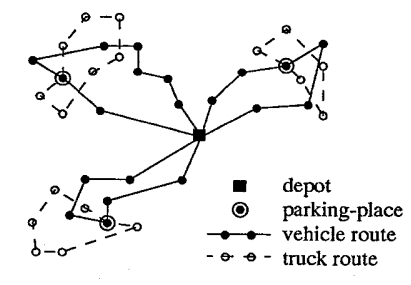
\includegraphics[width=0.5\textwidth]{Images/fig7.png}
\caption{Notacion de las rutas por Gerdessen ~\cite{Gerdessen}} 
\end{figure}

Gerdessen en su artículo propone una serie de heurísticas que se encargan de encontrar soluciones ``buenas'' para el VRPT en un tiempo razonable. Estas heurísticas pueden ser separadas en: 3 heurísticas para la construcción de una solución inicial y una de heurística de mejoramiento de soluciones ~\cite{Gerdessen} . Estas han sido utilizadas hasta el día de hoy para la construcción de soluciones. Luego en el año 2002 ``nace'' el problema de enrutamiento de camiones y trailers de mano de I-Ming Chao.
Chao en su investigación aborda el problema de la siguiente manera, usa las bases y supuestos de Gerdessen, es decir, notaciones y algunas de las restricciones. Para generar las soluciones iniciales Chao usa lo que denomina semillas, es decir los clientes que estén más alejados del centro de despacho, además en su modelo propuesto donde su variable es el si se asigna o no un cliente i a la ruta del camión j. Cada cliente es asignado a uno de los tres tipos de ruta, una ruta de camiones puro solamente v.c o t.c y una ruta de vehículos puros solamente de tipo v.c, los cuales pueden ser tratados como un problema del vendedor viajero. Para convertir  las soluciones infactibles en factibles Chao ~\cite{Chao} utiliza lo que el llama pasos de mejora independiente, los cuales son OPD, OTP, redefinición de raíz de un sub-tour y para reducir un poco la distancia se usa el movimiento 2-opt. Para la resolución del problema, Chao utiliza la búsqueda tabú ~\cite{Glover} con dos heurísticas, la restricción tabú basada en frecuencia y la desarrollada por ellos mismos, la restricción tabú basada en objetivos, en conjunto con los métodos ODP y TDP.
%Mencionar lo de las semillas
%luego sobre los pasos conr\strucion mejora y OPD TPD
%luego sobre los resultados


Para poder probar las heurísticas usadas y propuestas Chao utilizó los problemas VRP propuestos por Christofides, Mingozzi, and Toth ~\cite{CMT} y los transformaron a problemas TTRP, para cada problema CMT tres TTRPs son creados.

\begin{figure}[hp!]
\label{Tabla3}
\centering
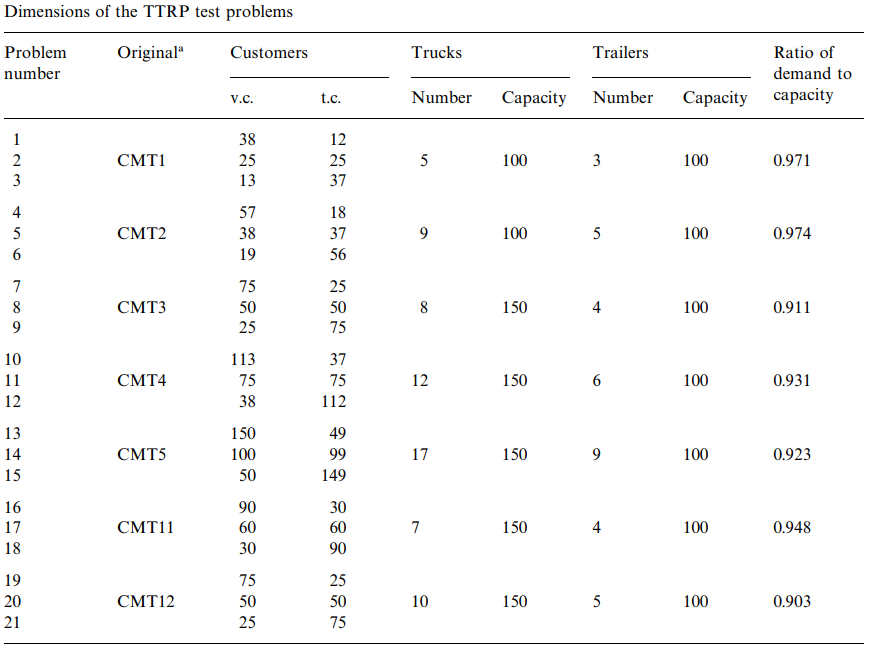
\includegraphics[width=0.75\textwidth]{fig2.png}
\caption{Tabla con las instancias de los problemas usados por Chao ~\cite{Chao}} 
\end{figure}

La ejecución de la heuristica de Chao TSTTRP fue desarollada en FORTRAN 5.0, sin embargo no se dice la representación usada, pero se intuye que se usa 2 arreglos bi-dimensionales, uno para las rutas principales y otro para los sub-tours. A continuación se presentan los resultados obtenidos por Chao:

\begin{figure}[htbp!]
\label{Tabla1}
\centering
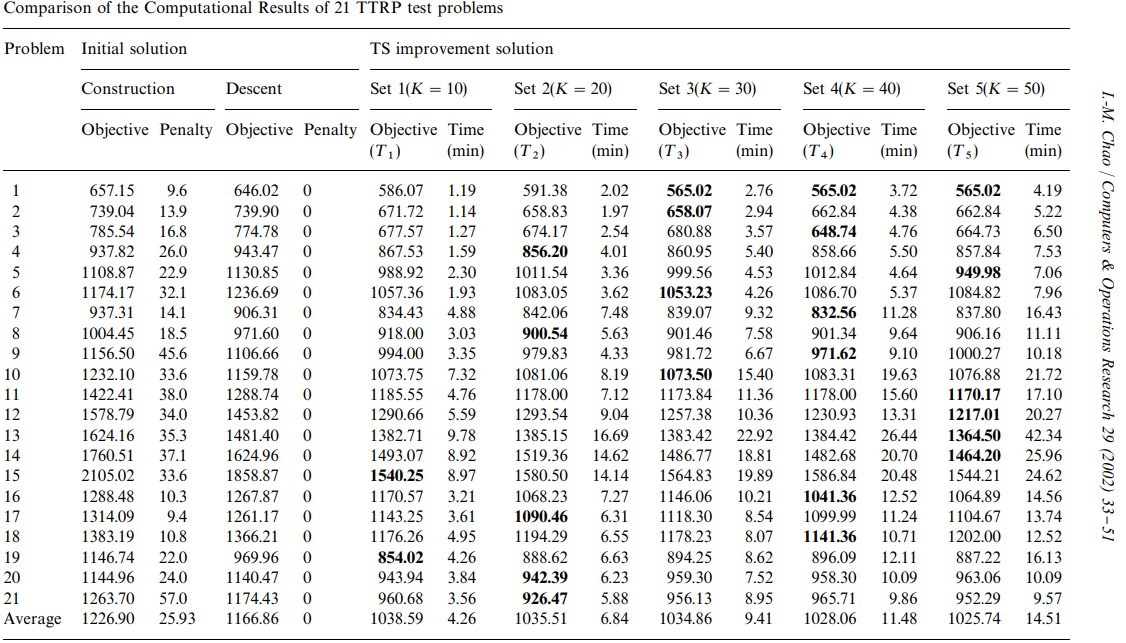
\includegraphics[width=0.85\textwidth]{fig3.png}
\caption{Tabla con las tiempos computacionales que obtuvo Chao ~\cite{Chao}} 
\end{figure}

\begin{figure}[htbp!]
\label{Tabla2}
\centering
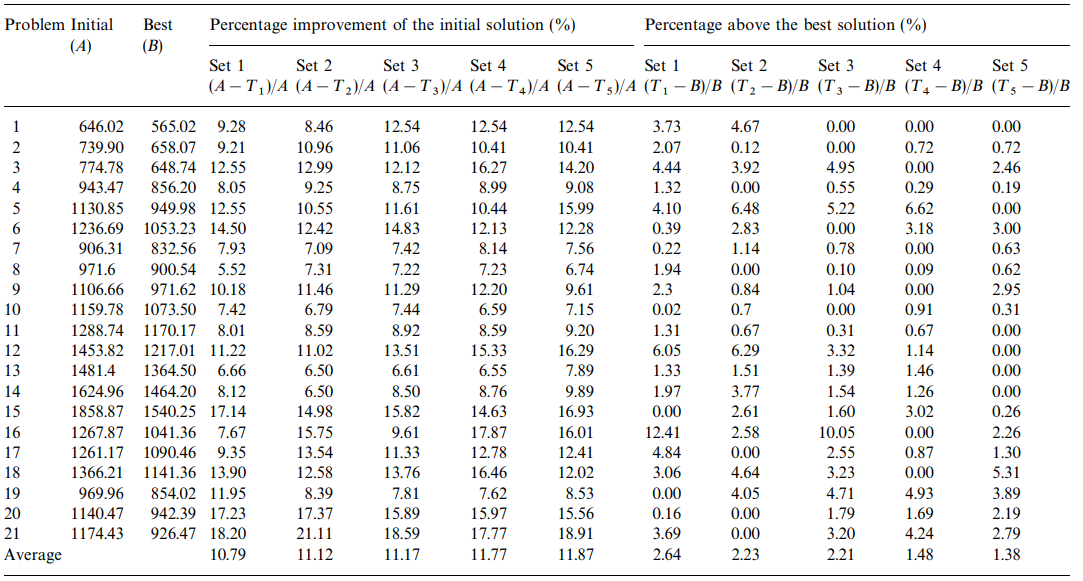
\includegraphics[width=0.85\textwidth]{fig4.png}
\caption{Tabla con las mejoras de resultado que obtuvo Chao ~\cite{Chao}} 
\end{figure}

%hablar de  como villega llego al resultado y sus representaciones
Estos resultados algunos investigadores los han usado para comparar sus propias heurísticas e investigaciones. Un ejemplo de ello es la investigación que realizaron Villegas et al. ~\cite{Villegas}, ellos proponen una solución usando \textbf{GRASP} (Greedy randomized adaptative search procedures) con una búsqueda local iterada (\textbf{ILS}), propuesto por primera vez por Prins ~\cite{GRASP}. Ellos obtuvieron los siguientes resultados al aplicar su propuesta de metaheuristica, sin embargo analizaron una variación, RTTRP, junto con realizar una comparativa de su propuesta con los otros métodos que se han propuesto para resolver RTTRP comparando con Chao ~\cite{Chao} y Lin et. al ~\cite{TTRPTW}(Figura 5).

\begin{figure}[htbp!]
\label{Tabla4}
\centering
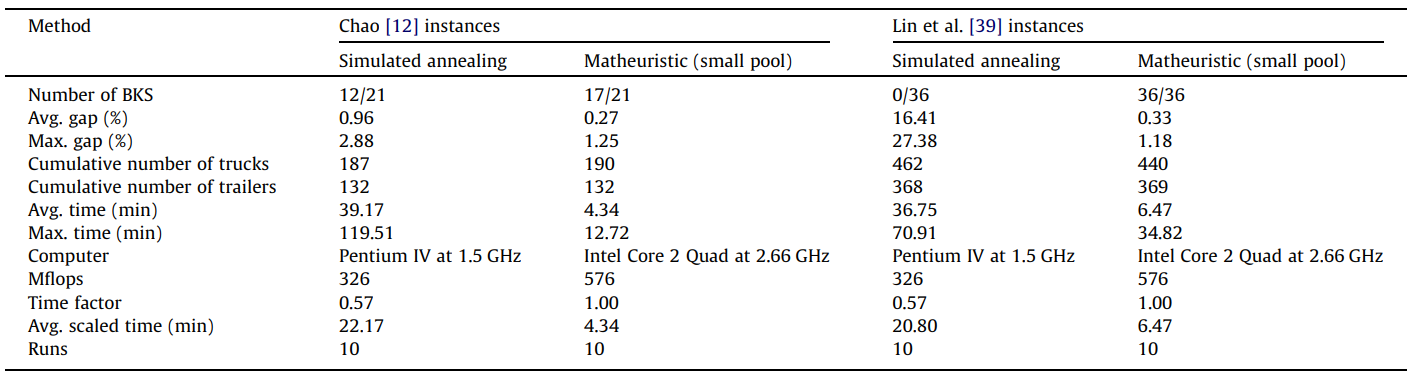
\includegraphics[width=0.85\textwidth]{Images/fig8.png}
\caption{Tabla con las comparativas de  Chao y Lin ~\cite{Villegas}} 
\end{figure}

\begin{figure}[htbp!]
\label{Tabla5}
\centering
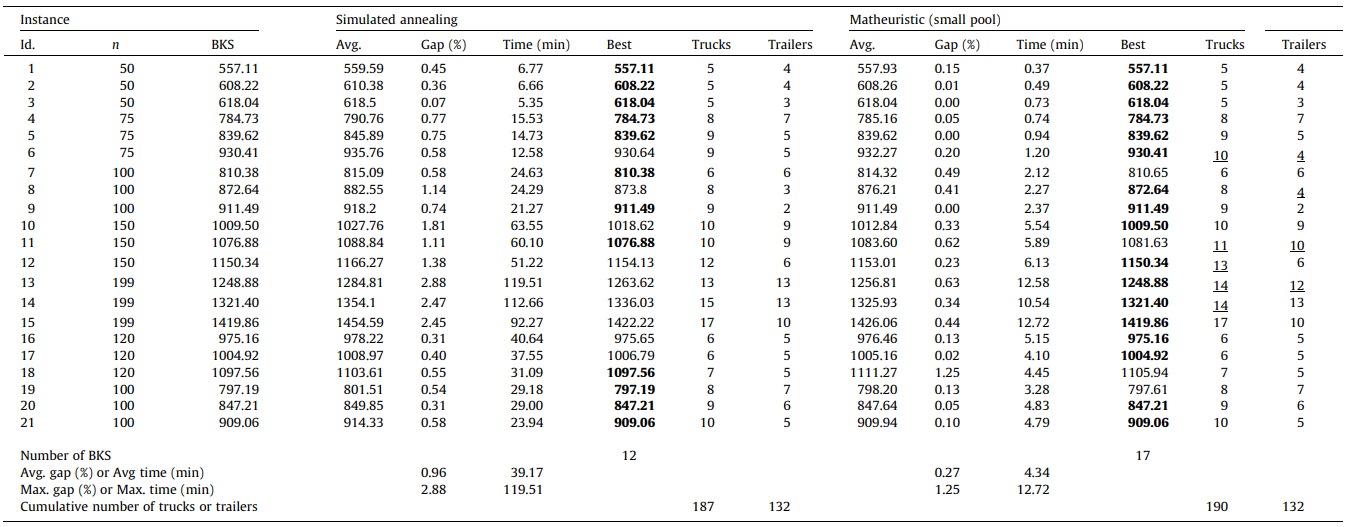
\includegraphics[width=0.85\textwidth]{Images/fig6.png}
\caption{Tabla con las comparativas de Villegas et al. con Chao ~\cite{Villegas}} 
\end{figure}

\begin{figure}[htbp!]
\label{Tabla5}
\centering
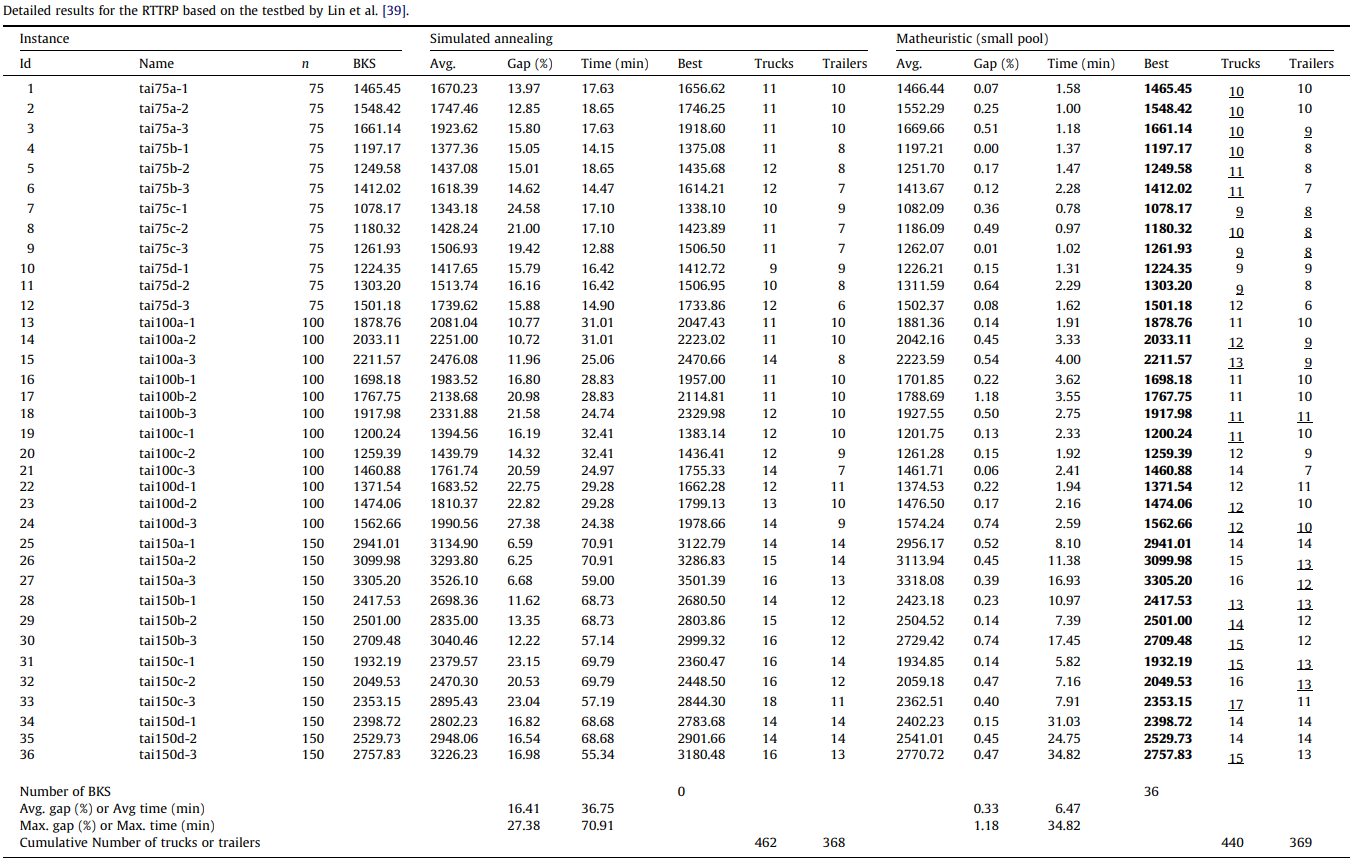
\includegraphics[width=0.85\textwidth]{Images/fig9.png}
\caption{Tabla con las comparativas de Villegas et al. con Lin ~\cite{Villegas}} 
\end{figure}

Villegas et al ~\cite{Villegas} obtiene los mismos valores de la función objetivo que Chao ( Figura 6), pero con un tiempo computacional menor y en algunos casos usando una cantidad mayor de camiones y trailers que los instanciados por Chao, por lo que la propuesta de Villegas tiene un mejor desempeño que la forma de trabajar de Chao. En el caso de Lin, Villegas obtiene mejores soluciones y con un tiempo  de ejecución mucho menor que Lin (figura 7).

Este problema tiene una tendencia a seguirse tratando y basándose en los supuestos que Gerdessen propuso. Sin embargo con el avance de la computación, puede que estos problemas se resuelvan de una manera más rápida, como efecto de los mejores procesadores  y GPUs que existen en la actualidad. Además que  este problema es un punto fundamental de la logística de las empresas que se especializan o que su mercado es la mensajería y entrega de encomiendas. 

\section{Modelo Matem\'atico}
\label{modelo}

Uno de los modelos propuestos para este problema fue hecho por Chao ~\cite{Chao}:
Sea $V = \{0,1,2,...,n\}$ el conjunto de nodos de nuestra red, siendo el nodo 0 el centro de distribución y $E$ el conjunto de caminos que conectan a los nodos. Cada nodo posee una demanda positiva $q_i, \forall i \in V - \{0\}$ y cada camino tiene un costo simétrico y no negativo $c_{ij} \in E$ donde $c_{ij}$ es la distancia euclidiana entre los nodos. Sea $d_{ij}= c_{0i}+c_{is_j}+c_{0s_j}$ el costo de asignar el cliente $i$ a la ruta $j$ ya sea de camión o vehículo, donde $s_j$ es la semilla de la ruta $j$.

\begin{align}
min &\sum_{i=1}^{n} \sum_{j=1}^{m_k} d_{ij}x_{ij}\\
\text{s.a } &\sum_{j=1}^{m_k} x_{ij} = 1, i = 1,2,...,n\\
\sum_{i=1}^{n} &q_ix_{ij} \leq Q_l + Q_k,  j = 1,2,...,m_l\\
\sum_{i=1}^{n} &q_ix_{ij} \leq Q_k,  j = 1,2,...,m_k,\\
x_{ij} &= \{0,1\}, i=1,2,...,n ,  j = 1,2,...,m_k\\
0 &\leq x_{ij}, i=1,2,...,n ,  j = 1,2,...,m_k
\end{align}

La función objetivo (1) representa la minimización del costo total de la asignación, por su parte las restricciones (2) y (5) establecen que un cliente puede estar en una sola ruta. La restricción (3) limita la carga que puede llevar un vehículo, es decir que la demanda de la ruta asignada debe ser menor o igual a la capacidad que tiene el camión más el trailer. De similar manera la restricción (4) limita que la demanda de la ruta debe ser menor o igual a la capacidad del camión. La restricción (6) establece que los valores de las variables pueden ser mayores o iguales a 0, por lo que induce soluciones infactibles, pero que después se pueden mejorar. Y lo más importante, la variable $x_{ij}$ indica si se asigna el cliente i a la ruta j.

Cabe destacar que el modelo propuesto por Chao no busca solucionar el problema, si no que poder generar soluciones iniciales ya sean factibles o no, para luego ser mejoradas con sus métodos ~\cite{Chao}. 
El espacio de búsqueda que tendría este problema seria de $2^{n * mk}$.


\section{Representaci\'on}
Para la representación de la solución se usa un arreglo bidimensional de tamaño $n \times m$ donde $n$ es la cantidad de rutas en total, es decir rutas y sub-rutas y $m$ es la cantidad de clientes pertenecientes a la ruta. La estructura de datos que se usará es un vector de vectores de números enteros con la siguiente interpretación, la posición del vector de enteros en el vector de vectores es el número de ruta creada y la posición de los números enteros en el vector de números enteros es el orden de visita, es decir el que esta en el índice 1, es el que se visita primero después de salir del centro de distribución o el que se visita después de desacoplar el trailer y así sucesivamente hasta llegar al $n-1$ que es el ultimo que se visita antes de volver al centro de distribución o volver al nodo raíz de la sub ruta. 

\section{Descripci\'on del algoritmo}
Las instancias que se usarán para resolver el problema tienen la siguiente estructura:
\begin{verbatim}
    n_camiones capacidad_camiones n_trailers capacidad_trailes n_clientes
    0 posx posy demanda tipo
    .
    .
    .
    n_clientes posx posy demanda tipo
\end{verbatim}
Una consideración a tener aunque igual se explica en las secciones anteriores es que el centro de distribución siempre será el ``cliente'' 0, además este no tendrá demanda alguna. El siguiente algoritmo que se presenta, es el algoritmo que se encarga de la lectura de las instancias.
\begin{algorithm}
\caption{Read instances}\label{lectura_instances}
\begin{algorithmic}[1]
\Procedure{Read}{$file$,\&n\_cam,\&n\_tra,\&cap\_cam,\&cap\_tra,\&n\_cli}\Comment{solamente el archivo es pasado directamente, los demás parámetros son por referencia}
    \State $\text{line}\gets  getline(file)$ 
    \State $\text{n\_cam,cap\_cam,n\_tra,cap\_tra,n\_cli}\gets line$
    \State $ clientes \gets vector<Cliente>$ \Comment{Cliente es una estructura que guarda los datos}
\While{!getline(file)}\Comment{Mientras no sea el fin del archivo}
    \State Cliente cliente
    \State $\text{line}\gets  getline(file)$ 
    \State $\text{cliente.numero,cliente.posx,cliente.posy,cliente.demanda,cliente.tipo}\gets line$
    \State $clientes\gets cliente$
\EndWhile\label{Lectura}
\State \textbf{return} $clientes$
\EndProcedure
\end{algorithmic}
\end{algorithm}

La estructura de datos mencionada $Cliente$ es una estructura que contiene los datos de un cliente es decir, contiene su numero de cliente, su posición en el eje x, su posición en el eje , la demanda que el cliente tiene y el tipo es decir si es un cliente t.c o v.c.

Luego de obtener los datos se calcula la matriz de costos, es decir la matriz con la distancia euclidiana entre todos los puntos. Una vez obtenida la matriz se calcula lo que se de nomina semillas, estas semillas según Chao ~\cite{Chao} son los puntos más lejanos que crearán las rutas. El procedimiento para generar las semillas es el siguiente: primero se elige el nodo más lejano respecto al centro de distribución, luego se elige el segundo mas lejano del centro de distribución y las semillas. Esto se hace la misma cantidad de veces que camiones disponibles haya.

Una vez obtenidas las semillas se calcula $d_{ij}$, el cual es el mismo que usa Chao ~\cite{Chao} para resolver un problema de asignación para generar la solución inicial. Luego de eso se realiza HC con MM para la búsqueda de soluciones.

\begin{algorithm}
\caption{Generate Solution}\label{generar soluciones}
\begin{algorithmic}[1]
\Procedure{Solve}{clientes,IT\_MAX,n\_cam}
\State  Costos $\gets$ euclideanMatrix(clientes)
\State   dijMatrix $\gets$ dijmatrix(Costos, n\_cam)
\State Sol\_ini $\gets$ ASPRO(dijMatrix)
\State sea N Vector de vecinos
    \While{$i<IT\_MAX$}
        \State Vecino $\gets$ swap(Sol\_ini)
        \If {len(N) $<$ n\_clientes/2}
        \State Sol\_ini $\gets$ Minimun(N)
        \State Empty(N)
        \EndIf
    \EndWhile
\EndProcedure
\end{algorithmic}
\end{algorithm}

El algoritmo descrito indica la forma en que se obtendrá la solución inicial. La función euclideanMatrix obtiene la matriz de costos del problema, dij\_Matrix indica cuales son las rutas que se crearon y cual es el costo de agregar a los clientes a aquella ruta. La función ASPRO se encarga de generar la solución inicial que será utilizada para la generación del vecindario de las soluciones.


%Secci\'on Referencias: Indicando toda la informaci\'on necesaria de acuerdo al tipo de documento revisado. Las referencias deben ser citadas en el documento.
\bibliographystyle{plain}
\bibliography{Referencias}
\end{document} 
